%\documentclass[conference]{IEEEtran}
\documentclass{sig-alternate}
\usepackage{datatool}
%\usepackage{amsthm}
\usepackage{booktabs}
\usepackage{graphicx}
\usepackage{enumerate}
\usepackage{cprotect}
\usepackage{xtab}
\usepackage{tikz}
\usepackage{url}
\usepackage[update,prepend,outdir=./]{epstopdf}
\DTLsetseparator{•}
\DTLloaddb{data}{../analysis_output/database.csv}

\usepackage{cite}
\usepackage{balance}

%submission site: http://cyberchairpro.borbala.net/asepapers/submit/
% Login: carl1978@iastate.edu
% Password: ASE-143111797041267

\widowpenalty=10000
\clubpenalty=10000

\newcommand{\todoNow}[1]{\textbf{\textcolor{red}{TODO.NOW: #1}}} %comment out for submission
\newcommand{\todoMid}[1]{\textbf{\textcolor{green}{TODO.MID: #1}}} %comment out for submission
\newcommand{\todoLast}[1]{\textbf{\textcolor{blue}{TODO.LAST: #1}}} %comment out for submission
\newcommand{\yes}{\tikz\draw[black,fill=black] (0,0) circle (.5ex);}
\newcommand{\sorta}{\tikz\draw[gray,fill=gray] (0,0) circle (.5ex);}
\newcommand{\no}{\tikz\draw[black] (0,0) circle (.5ex);}


\newtheorem{mydef}{Definition}

\begin{document}
%
% paper title
% can use linebreaks \\ within to get better formatting as desired
%\title{Regex Feature Use In Practice}
\title{Regular Expression Feature Usage in Python}

% author names and affiliations
% use a multiple column layout for up to three different
% affiliations
\numberofauthors{2}

\author{
\alignauthor
Carl Chapman\\
       \affaddr{Department of Computer Science}\\
       \affaddr{Iowa State University}\\
       \affaddr{Ames, IA, USA}\\
      \email{carl1978@iastate.edu}\\
 \alignauthor
Kathryn T. Stolee\\
       \affaddr{Departments of Computer Science and}\\
             \affaddr{Electrical and Computer Engineering}\\
       \affaddr{Iowa State University}\\
       \affaddr{Ames, IA, USA}\\
      \email{kstolee@iastate.edu}\\
}

% make the title area
\maketitle


\begin{abstract}
Regular expressions are used frequently in programming languages for form validation, ad-hoc file searches, and simple parsing. Due to the popularity and pervasive use of regular expressions, researchers have created tools to support their creation, validation, and use. Each tool has made design decisions about which regular expression features to support, and these decisions impact the usefulness and power of the tools. Yet, these decisions are often made with little information as there does not exist an empirical study of regular expression feature usage to inform these design decisions.

In this paper, we survey 18 professional developers about the context and frequency of their regular expression usage. Then, we
explore regular expression feature usage in Python, focusing on how often features are used and the diversity of regular expressions from syntactic and semantic perspectives. We analyzed nearly 4,000 open source Python projects from GitHub and extracted nearly 14,000 unique regex patterns that were used for analysis.
We also map the most common features used in regular expressions to those features supported by four common regex engines from industry and academia, brics, Hampi, Re2, and Rex.
Our results indicate that developers frequently use regular expressions in their programming practices, but often those regular expressions do not persist (e.g., when used for command line or file search purposes). For regular expressions found in Python projects,
the most commonly used features are also supported by popular research tools and that programmers frequently reinvent the wheel by writing identical or nearly identical regular expressions in different ways.
We conclude by discussing the implications for  tool  designers and outline several directions of future work.
%FYI: nProjScanned = 3898
%These observations lead to suggestions on which regular expression features are imperative to support and for future directions in research to help developers write and reuse regular expressions.
\end{abstract}

\section{Introduction }

Regular expressions (regexes) are an abstraction of keyword search that enables the identification of text using a pattern instead of an exact keyword.
Regexes are commonly used for parsing text, form validation, and text searching within text editors (e.g., emacs), command line tools (e.g., grep, sed) and IDEs (e.g., the search feature in the Eclipse IDE).  Although regexes are powerful and versatile, they can be hard to understand,  maintain, and debug, resulting in tens of thousands of bug reports~\cite{Spishak:2012:TSR:2318202.2318207}.

Due in part to their common use across programming languages and how susceptible regexes are to error, many researchers and practitioners have developed tools to support more robust creation~\cite{Spishak:2012:TSR:2318202.2318207} or to allow visual debugging~\cite{Beck:2014:RVD:2591062.2591111}. To remove the human in the loop, other research has focused on learning regular expressions from  text~\cite{Babbar:2010:CBA:1871840.1871848, Li:2008:REL:1613715.1613719}.
Beyond supporting regular expression usage, the applications of regular expressions in research include test case generation~\cite{Ghosh:2013:JAT:2486788.2486925, Galler:2014:STD:2683035.2683100, Anand:2013:OSM:2503903.2503991, Tillmann:2014:TAT:2642937.2642941},
specification for string constraint solvers~\cite{Trinh:2014:SSS:2660267.2660372, hampi}, and as queries in a data mining framework~\cite{Begel:2010:CDE:1806799.1806821} or on the semantic web~\cite{Lee:2010:PSQ:1871871.1871877}.
Regexes are also employed in critical missions like mysql injection prevention~\cite{Yeole:2011:ADT:1980022.1980229} and network intrusion detection~\cite{network}, or in more diverse applications like DNA sequencing alignment~\cite{1594922}.

These researchers and tool designers must pick what features to include or exclude, which  can be a difficult  design decision. Supporting advanced features may be more expensive, taking more time and potentially making the project too complex and cumbersome to execute well.  A selection of only the simplest of regex features limits the applicability or relevance of that work. Despite extensive research effort in the area of regex support,  no research has been done about how regexes are used in practice and what features are essential for the most common use cases.


\emph{The goal of this work is to explore 1) the context in which developers use regular expressions, and 2) the features and diversity of  regular expressions found in Python projects}.
First, we survey developers about the context of their regex usage, include how often and for what purposes regexes are composed.
Second, we measure how often regex features (e.g., kleene star, character classes, and capture groups are all features) appear in regular expressions and used in Python projects.
By comparing the features to those supported by four common regex support tools, brics~\cite{brics}, hampi~\cite{hampi}, Rex~\cite{rex}, and RE2~\cite{re2} and surveying developers about some of the less supported feature, we discuss the potential impact of omitting various features.
Third, using  a semantic analysis to cluster similar regular expressions that occur in multiple projects, we explore the most common behaviors captured by  regexes in Python.
Our results indicate that regexes are most frequently used in command line tools and IDEs, that capturing the contents of brackets and searching for delimiter characters were some of the most specific cluster behaviors, and that the capture group feature and the endpoint anchor features are the most widely used features that are poorly supported in regex tools.
The contributions of this work are:
\begin{itemize}
    \item A survey of 18 professional software developers about their experience with regular expressions,
	\item An empirical analysis of regex feature usage of nearly 14,000 regular expressions in \DTLfetch{data}{key}{nProjScanned}{value} open-source Python projects, mapping of those features to those supported by common regex tools and survey results showing the impact of not supporting various features,
	\item An approach for measuring semantic similarity of regular expressions and qualitative analysis of the most common semantically similar clusters, and
	\item A discussion of opportunities for future work in supporting programmers in writing regular expressions.
\end{itemize}

The rest of the paper is organized as follows. Section~\ref{sec:related} motivates this work by discussing research in supporting programmers in the use, creation, and validation of regular expressions. Section~\ref{sec:study} presents the research questions, survey design, and study setup for exploring regular expressions in the wild. Results of these explorations are in Section~\ref{sec:results} followed by a discussion in Section~\ref{sec:discussion}. Threats to validity are in Section~\ref{sec:threats} and the conclusion is in Section~\ref{sec:conclusion}.


\section{Related Work}
\label{sec:related}

%To improve test coverage for code using regular expressions, and to generate strings from regular expressions for whatever other reasons, projects like Reggae~\cite{rex}, Rex~\cite{rex}, JST~\cite{rex}, regex-tester\footnote{\url{https://github.com/nickawatts/regex-tester}}, regldg\footnote{\url{http://regldg.com/}}, uttool\footnote{\url{http://uttool.com/text/regexstr/default.aspx}}, xeger\footnote{\url{https://code.google.com/p/xeger/}}, Generex\footnote{\url{https://github.com/mifmif/Generex}}, Hoa/Regex\footnote{\url{https://github.com/hoaproject/Regex/}}, Genex\footnote{\url{http://search.cpan.org/~bowmanbs/Regexp-Genex-0.07/lib/Regexp/Genex.pm}}, Randexp\footnote{\url{https://www.ruby-toolbox.com/projects/randexp}}, txt2re\footnote{\url{http://txt2re.com/}}, Pex\footnote{\url{http://research.microsoft.com/en-us/projects/pex/}}  have been developed.

%
%Going the other direction, a few projects have attempted to take a set of strings and generate a good regular expression that matches them like RegexGenerator++\footnote{\url{http://regex.inginf.units.it/}} and Regex-PreSuf\footnote{\url{http://search.cpan.org/~jhi/Regex-PreSuf-1.17/PreSuf.pm}} (a problem that suffers from overmatching).
%%Tools to help developers write correct regular expressions, tools like RegexBuddy, Expresso, Pythex, The Regex Coach, Regex Widget, Regex magic, RegE xr, reWork, Rubular, Txt2re and....

\todo{do we want to include the commented list or not?}

One common misconception is that all regular expression languages are \emph{regular languages} which can be represented using deterministic finite automata (DFA), and so they are easy to model, easy to describe formally and execute in O(n) time.  In fact, many regular expression matching engines run in exponential time in order to support useful features such as lazy quantifiers, capturing groups, look-aheads and back-references~\cite{msdnmatching}.  In the RE2 projext~\cite{re2}, Russ Cox aimed to use DFAs as much as possible (maximizing speed) while supporting as many useful features as possible.

%Thousands of research papers have focused on various other regular expression-related investigations.
Since  regular expression languages vary somewhat in their syntax and feature set, researchers and tool designers have typically had to describe a particular language to reason about and have had to pick what features to include or exclude. Researchers and tool designers face a difficult design decision: supporting advanced features is always more expensive, taking more time and potentially making the tool or research project too complex and cumbersome to execute well.  A selection of only the simplest of regex features is common in research papers and automata libraries, but this limits the applicability/relevance of that work in the real world.



In this work, we perform a feature analysis on regular expressions used in the wild and compare that set to the features supported by four popular regular expression tools.
Research tools like Hampi~\cite{hampi}, and Rex~\cite{rex}, and commercial tools like brics\cite{brics} and RE2~\cite{re2}, all use regular expressions for various task. Hampi was developed  in academia and uses regular expressions as a specification language for a strong constraint solver. Rex was developed by Microsoft Research and generates strings for regular expressions that can be used in several applications, such as test case generation~\cite{}. Brics is an open-source package that creates automata from regular expressions for manipulation and evaluation.
While there are many regular expression tools available, in this work, we focus on the features support for these four tools, which offer diversity across developers (i.e., Microsoft, Google, open source, and academia) and across applications. Further, as the focus of this work is on tool designers, these four tools and their features are well-documented, allowing for easy comparison.


% \subsection{Research on Regular Expressions}
% Visual debugging of regular expressions~\cite{Beck:2014:RVD:2591062.2591111}

% %the related work section in the Spishak section is very good re: regex tools like those that represent regexes as automata or grammars
% Static analysis to reduce errors in building regular expressions by using a type system to identify errors like {\tt PatternSyntaxExceptions} and {\tt IndexOutOfBoundsExceptions} at compile time~\cite{Spishak:2012:TSR:2318202.2318207}.

% \subsection{Research on Regular Expressions}
% Visual debugging of regular expressions~\cite{Beck:2014:RVD:2591062.2591111}

% \subsection{Research that Depends on Regular Expression Usage}
% Regular expressions are used as queries in a data mining framework~\cite{Begel:2010:CDE:1806799.1806821}



\section{Survey}
\label{sec:survey}

To understand the context of when and how programmers use regular expressions,
we designed a survey with 41 questions about regex usage. This survey was
deployed to developers at Dwolla, a company that provides software for
 online and mobile payment management.
 \todoLast{they are probably ok with using their name - check during final scrub by Dwolla}
Participation was voluntary and participants were entered in a lottery for a \$50 gift card.
The survey was completed by 18 participants that identified as software developer/maintainers who had used regular expressions in a work environment.


On average, survey participants report to compose 172 regexes per year ($\sigma$ = 250) and compose regexes on average once per month, with 27\% composing multiple regexes in a week and an additional 22\% composing regexes once per week.
Table~\ref{tab:regexenviron} shows how frequently participants compose regexes using each of several languages and technical environments.
Six (33\%) of the survey participants report to compose regexes using general purpose programming languages (e.g., Java, C, C\#) 1-5 times per year and 5 (28\%) do this 6-10 times per year.  Regexes were rarely used in query languages like SQL, but for command line usage in tools such as grep, 6 (33\%) participants use regexes 51+ times per year. Overall, regexes are used frequently, but in some environments, such as command line or text editor, and sometimes query languages, the composed regular expressions do not persist.

\newcommand{\horiz}{\hspace{2.1pt}}

\begin{table}
\caption{Survey results for number of regexes composed per year by technical environment \label{tab:regexenviron}}
\begin{center}
\begin{small}
\begin{tabular}{l | r @{  \horiz} r @{ \horiz } r @{ \horiz } r @{ \horiz } r @{ \horiz } r }
Language/Environment & 0 & 1-5 & 6-10 & 11-20 & 21-50 & 51+ \\ \hline
General  (e.g., Java)  & 1 & 6 & 5 & 3& 1& 2 \\
Scripting  (e.g., Perl) &5 &4 &3 &3 &2  &1 \\
Query  (e.g., SQL) & 15&2 &0 &0 &1  & 0\\
Command line (e.g., grep)   &2 &5 &3 &2 &0  &6 \\
Text editor (e.g., IntelliJ)   & 2& 5& 0& 5& 1& 5\\
\end{tabular}
\end{small}
\end{center}
\end{table}

\begin{table}
\caption{Survey results for regex usage frequencies for various activities, averaged using a 6-point likert scale: Very Frequently=6, Frequently=5, Occasionally=4, Rarely=3, Very Rarely=2, and Never=1 \label{tab:regexactivities}}
\begin{center}
\begin{tabular}{l|c}
Activity & Frequency \\ \hline
Locating content within a file or files & 4.4\\
Capturing parts of strings & 4.3 \\
Parsing user input & 4.0\\
Counting lines that match a pattern & 3.2\\
Counting  substrings that match a pattern & 3.2\\
Parsing generated text & 3.0\\
Filtering collections (lists, tables, etc.) & 3.0 \\
Checking for a single character & 1.7\\


\end{tabular}
\end{center}
\end{table}

Table~\ref{tab:regexactivities} shows how frequently, on average, the participants use
regexes for various actives.
Participants answered questions using a 6-point likert scale including very frequently, frequently, occasionally, rarely, very rarely, and never.
Assigning values from 1 to 6, where 6 is the most frequent, the responses were averaged across participants.
\todoLast{is the 6-point scale overemphasized here and in the table caption?}
Among the most common are capturing parts of a string and locating content within a file, with both occurring somewhere between occasionally and frequently.

Using a similar 7-point likert scale that includes 'always' as a seventh point, developers indicated that they test their code with the same frequency as they test their regexes (5.2 which is between frequently and very frequently).  Half of the 18 developers indicate that they use tools to test their regexes, and the other half indicated that they only use tests that they write themselves. Of the 9 developers using tools, 6 of them mentioned some online composition aide similar to regex101.com where a regex and input are entered, and the input is highlighted according to what is matched.
%The other three developers mentioned 'ScalaCheck' (a testing framework), 'IDE regex plugins', and 'Language specific Regexlib'.

When asked an open ended question about pain points encountered with regular expressions, 7 developers responded with an answer equivalent to 'hard to read', 3 responded with 'inconsistency across implementations' and 11 responded with 'hard to compose' (3 developers gave two answers).

The survey validates the assumption that regex are widely used by professional software developers.  Future research into regex can focus on areas that prove to be most important to developers, namely capturing parts of strings and searching for specific content.  Although research into regex use in general purpose and scripting languages is important, usage within command line tools and text editors should also be considered.  The fact that all the surveyed developers compose regexes, and half of the developers use tools to test their regexes indicates the importance of tool development for regex.  Developers complain about regex being hard to read and hard to compose, and most of the tools that they indicate using are focused on composition, indicating a need for tools that help make existing regexes more readable.


\section{Study}
\label{sec:study}

To understand how programmers use regular expressions in Python projects, we scraped \DTLfetch{data}{key}{nProjScanned}{value} Python projects from GitHub, and recorded regex usages for analysis as described in Section~\ref{study:corpus}.
Throughout the rest of this paper, we  employ the following terminology:

\noindent \textbf{Utilization}: A \emph{utilization} occurs whenever a developer uses a regex engine in a project.  Within a particular file in a project, a \emph{utilization} is composed of a function, a pattern and 0 or more flags.  Figure~\ref{fig:exampleUsage} presents an example of one regex \emph{utilization}, with key components labeled. The function called from the {\tt re} module is {\tt re.compile} does \todo{describe this module}, the pattern observed (i.e., a regex string) is {\tt `(0 $\mid$-?[1-9][0-9]*)\$'} represents strings with \todo{briefly describe the regex}, and the flag allows string matching over multiple lines.
Thought of another way, a regular expression  utilization is one single invocation of the {\tt re} library in a project.

\begin{figure}[htb]
\centering
\includegraphics[width=\columnwidth]{../illustrations/exampleUsage.eps}
\caption{example of one regex utilization}
\label{fig:exampleUsage}
\end{figure}



\noindent \textbf{Pattern}: A \emph{pattern} is an ordered series of regular expression language feature tokens that can be used to find match start and end indices within an input string.  Notice that because the vast majority of regex features are shared across most all-purpose languages, a Python \emph{pattern} will (almost always) behave the same when used in Java, C\#, Javascript, Ruby, etc, whereas a \emph{utilization} is not universal in the same way (would not compile in other languages).

\subsection{Research Questions}
We aim to answer the following research questions:

\textbf{RQ1:} How  is the {\tt re} module used in Python projects?

To address this research question, we measure how often any calls are made to the {\tt re} module per file and per project in Python projects.

Furthermore, we measure the frequency of usage for calls to the 8 functions of the {\tt re} module ({\tt re.compile}, {\tt re.search}, {\tt re.match}, {\tt re.split}, {\tt re.findall}, {\tt re.finditer}, {\tt re.sub} and {\tt re.subn}) in Python projects scraped from GitHub.

We also measure usage of the 8 flags ({\tt re.DEFAULT}, {\tt re.IGNORECASE}, {\tt re.LOCALE}, {\tt re.MULTILINE}, {\tt re.DOTALL}, {\tt re.UNICODE}, {\tt re.VERBOSE} and {\tt re.DEBUG}) of the {\tt re} module.

Further, to provide context as to the overlap among regular expression strings used in Python, we explore the most common regex {patterns} across all utlizations.

\textbf{RQ2:} Which regex language features are most commonly used in python?

We consider regex language features to be tokens that specify the matching behavior of a regex pattern, like the {\tt +} in {\tt ab+}.  All studied features are coded and described in~\ref{study:corpus} with examples.

To measure feature usage, we parse Python regular expression patterns using Bart Kiers' PCRE parser, as described in Section~\ref{study:corpus}.  We then count the number of usages of each feature per project, per file and as a percent of all distinct regex patterns.

\textbf{RQ3:} What are Features being used for, and so what is the impact of \emph{not} supporting various regex features on tool designers and users?
%\textbf{RQ3:} What is the impact of \emph{not} supporting various regex features on tool designers and users?

We use semantic analysis to illustrate the impact of missing features on a tool's applicability, identifying what each feature (or group of features) is commonly used for.

Semantic analysis is accomplished by first establishing a similarity matrix between regexes using a set of strings that match each regex, generated by Rex.  Then clusters of regexes with similar behavior are discovered using Markov Clustering\footnote{\url{http://micans.org/mcl/}}.  These clusters are used to interpret what a feature is used for.

Since our semantic analysis is based on Rex, this semantic analysis cannot be applied to all features studied.  For these unsupported features, we use 6 string similarity metrics (Jaro-Winkler, Levenshtein, Longest Common Substring, Sift3, Jaccard and Cosine) to build similarity matrices.  As before, these matrices are used to find clusters of regexes, which are used to interpret what a feature is used for.

We chose Rex to build matching strings because it supports the most features of any String-generation tool.  We chose the mcl clustering tool because it offers a fast and tunable way to cluster items by similarity (without knowing the number of clusters in advance).



\subsection{Building the Corpus}
\label{study:corpus}
Github is a popular project hosting site containing over 100,000 Python projects.
We used the GitHub api to page through all repositories, cloning projects that contain Python code.

For each project, we used Astroid\footnote{\url{https://bitbucket.org/logilab/astroid}} to build the AST of each Python file and find \emph{utilizations} of Python's {\tt re} module.

Using git, each project was scanned at 20 evenly-spaced commits (or all commits if there were less than 20) in its history.
Within one project, we define a duplicate \emph{utilization} as a \emph{utilization} having the same function, pattern and flags within the same file (same relative path).  We ignored duplicate \emph{utilizations} to protect against over-counting the same \emph{utilization} as we rewind the project through its history.  We observed and recorded \DTLfetch{data}{key}{nUsages}{value} non-duplicate regex \emph{utilizations} in \DTLfetch{data}{key}{nProjScanned}{value} projects.

\subsection{Selecting Patterns}
Because the focus of this study is regex features,  analysis focuses on the patterns found, so we ignored the \DTLfetch{data}{key}{percentBadFlags}{value}\%  of \emph{utilizations} using flags that can alter regex behavior.  An additional \DTLfetch{data}{key}{percentInvalidPattern}{value}\% of \emph{utilizations} contained patterns that could not be compiled because the pattern was non-static (used some runtime variable), or because of other unknown parsing failures.

The remaining \DTLfetch{data}{key}{percentCleanUsages}{value}\% (\DTLfetch{data}{key}{nCleanUsages}{value}) \emph{utilizations} were collapsed into \DTLfetch{data}{key}{nDistinctPatterns}{value} distinct pattern strings.  The resulting set of patten strings were parsed using an antlr-based, open source PCRE parser released by Bart Kiers\footnote{\url{https://github.com/bkiers/pcre-parser}}.  This parser was unable to support \DTLfetch{data}{key}{percentUnicode}{value}\% (\DTLfetch{data}{key}{N_UNICODE}{value}) of the patterns due to unsupported unicode characters.  Another \DTLfetch{data}{key}{percentAlien}{value}\% (\DTLfetch{data}{key}{N_ALIEN}{value}) of the patterns used regex features that we have chosen to exclude in this study\footnote{\url{www.details.#thistopic}}.  The \DTLfetch{data}{key}{nCorpus}{value} distinct pattern strings that remain were each assigned a weight value equal to the number of distinct projects the pattern appeared in.  We will refer to this set of weighted, distinct pattern strings as the \emph{corpus}.

\subsection{Analyzing Features}
\label{study:features}

\todo{revise this subsection}
After picking four large regex research projects, the big table with the features was created in order to decide which unsupported features are used most often.
Our semantic analysis is dependent on the use of Rex to generate strings so we can identify semantically related clusters. For three common features unsupported by Rex, we rely on syntactic analysis to determine similarity among regular expressions containing those features. For those features supported by Rex, we cluster the regular expressions based on semantic diversity.

\subsubsection{Syntactic Diversity}
For the negative perspective, we picked three features: LZY, NCG, WNW that are unsupported by Rex and other projects.  For each of these features, we created a subset of the \emph{collection} where all the patterns contain that feature.  Then we used syntactic analysis...to create a similarity matrix.  We then used markov clustering [X] (MCL) to find clusters in the subset.  We used these clusters to assist our manual search for some common use cases for the unsupported feature.

Markov clustering can be tuned using many parameters, including inflation and filtering out all but the top-k edges for each node.  After exploring the quality of the clusters using various tuning parameter combinations\footnote{\url{www.details.#thistopic}}, the best clusters were found using an inflation value of 1.8 and k=83.

Note that the filteredCorpus is of size 9727, and at least one pattern from the fc can be found in 1375 of the original 3900 or whatever.  Most patterns do not belong in a cluster (for example a very specific pattern like \verb!<title>[^<]*Revision \d+:!), so after clustering is done only 2727 patterns are included, and only 999 projects have any of these patterns in them.


\subsubsection{Semantic Diversity}
For the positive perspective, we created another subset of patterns (XYZ patterns) where Rex was able to generate strings that the pattern matched.  We then created a similarity graph with weighted, undirected edges as shown in Figure~\ref{fig:similarityConstruction}.

\begin{figure}
\begin{description}
\setlength{\parskip}{0pt} % block paragraphs
\setlength{\itemindent}{0in}
\item for each row i:
\setlength{\itemindent}{0.2in}
\item obtain set of Rex-generated strings Ri from pattern at index i
\item sRi = size of Ri
\item for each col j:
\setlength{\itemindent}{0.4in}
\item Nij = number of strings in Ri matched by pattern at index j
\item M[i][j] = Nij/sRi
\setlength{\itemindent}{0in}
\item G = empty graph
\item for each row i:
\setlength{\itemindent}{0.2in}
\item for each col j:
\setlength{\itemindent}{0.4in}
\item SIMij = (M[i][j]+M[j][i])/2
\item if SIMij > 0.75:
\setlength{\itemindent}{0.6in}
\item add edge (i,j)=SIMij to G
\setlength{\itemindent}{0in}
\setlength{\parskip}{10pt} % block paragraphs
\end{description}
\caption{Constructing Similarity Graph \label{fig:similarityConstruction}}
\end{figure}

Again we used MCL to find clusters that aided a manual search for use cases strongly associated with particular features.













\section{Results}
\label{sec:results}

In this section, we present the results of each research question. 

\subsection{RQ1: How  is the {\tt re} module used in Python projects?}
To address this research question, we look at regex utilizations, flags, and the overlap among pattern strings among utilizations. 

\subsubsection{Saturation of Projects with Utilizations}
Out of the \DTLfetch{data}{key}{nProjScanned}{value}\ projects scanned, \DTLfetch{data}{key}{percentProjectsUsingRegex}{value}\% (\DTLfetch{data}{key}{nProjectsUsingRegex}{value}) contained at least one regex utilization.  For context about how saturated these projects were with utilizations, we consider how many utilizations were observed per project, how many files the average project scanned contained, how many of those files contained utilizations, and how many utilizations occurred per file in Table~\ref{table:saturation}.

The average regex utilizations per project was 32, but this is offset by a high maximum value of 1,427. This value appeared in a project that \todo{finish this sentence}. The average number of files containing a utilization was 11 out of the average total files per project of 53. On average, each file with a regex utilization had only two, with a median of 1. 


From Table~\ref{table:saturation}, we see that on average each project had \DTLfetch{data}{key}{medRFilePerProj}{value} files containing any regex usage, out of an average of \DTLfetch{data}{key}{medFilePerProj}{value} files.  Each of the files that did have a regex usage had an average of \DTLfetch{data}{key}{medRPerFile}{value} regex usages.  Because we scanned \DTLfetch{data}{key}{nProjScanned}{value} projects, we would expect to have seen \DTLfetch{data}{key}{nExpectedUsages}{value} regex usages, which is lower than the actual \DTLfetch{data}{key}{nUsages}{value} usages observed.

\begin{table}[tb]
\begin{center}
\begin{small}
\caption{How saturated are projects with utilizations? (RQ2)}
\label{table:saturation}

\begin{tabular}{l|ccccc}
\toprule
source & Q1 & Avg & Med & Q3 & Max \\ 
 \hline \bigstrut
utilizations per project & 2 & 32 & 5 & 19 & 1,427 \\ 
 \hline \bigstrut
files per project & 2 & 53 & 6 & 21 & 5,963 \\ 
 \hline \bigstrut
utilizing files per project & 1 & 11 & 2 & 6 & 541 \\ 
 \hline \bigstrut
utilizations per file & 1 & 2 & 1 & 3 & 207 \\ 
\bottomrule
\end{tabular}
\end{small}
\end{center}
\vspace{-12pt}
\end{table}


\subsubsection{Usage Frequency of {\tt re} Module Functions}

\begin{figure}[tb]
\centering
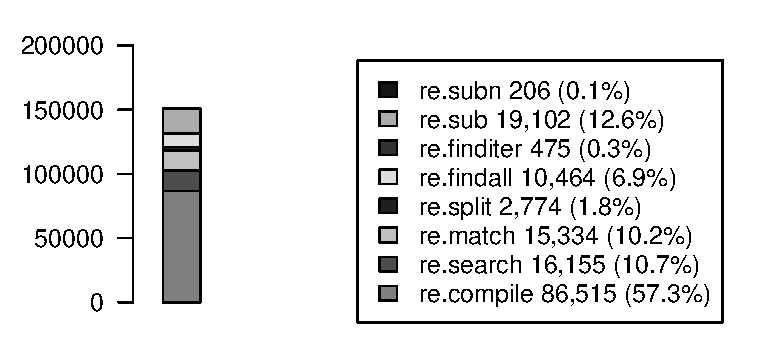
\includegraphics[width=\columnwidth]{../analysis_output/partFunctions.eps}
\caption{How often are the 8 re functions used? (RQ1)}
\label{fig:partFunctions}
\end{figure}

\begin{figure}[tb]
\centering
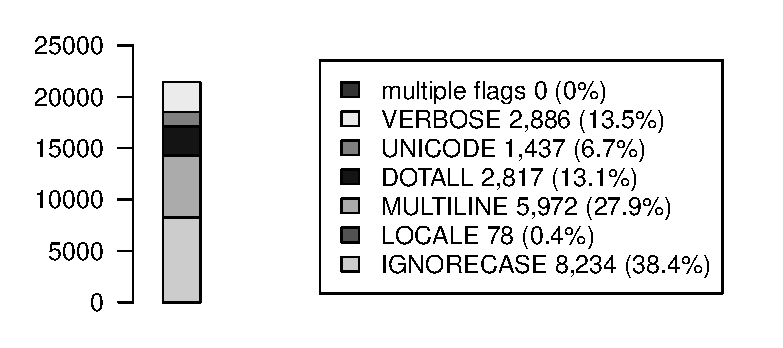
\includegraphics[width=\columnwidth]{../analysis_output/partFlags.eps}
\caption{Which behavioral flags are used? (RQ1)}
\label{fig:partFlags}
\end{figure}

The number of projects that use each of the {\tt re} modules are shown in Figure~\ref{fig:partFunctions}.  The y-axis denotes the total utilizations, with a maximum of \DTLfetch{data}{key}{nUsages}{value}. The {\tt re.compile} function encompasses \DTLfetch{data}{key}{percentCompile}{value}\% of all utilizations, presumably because each usage of those functions could accept the compiled regex as an argument. 

\subsubsection{Usage Frequency of {\tt re} Module Flags}
When considering flag use, we excluded non-behavioral flags (default and debug), which account for \DTLfetch{data}{key}{percentFlags0}{value}\% of all utilizations. \todo{are they both present in debug and default? how much of the 87\% is for each omitted flag? Why are these omitted, again?}

 As shown in figure ~\ref{fig:partFlags}, of all behavioral flags used, ignorecase (\DTLfetch{data}{key}{percentI}{value}\%) and multiline (\DTLfetch{data}{key}{percentM}{value}\%) were the most frequently used.  It is also worth noting that although multiple flags can be combined using a bitwise or, this was never observed.


\subsubsection{Most Frequently Observed Patterns}

\todo{need to describe these results}
Table~\ref{table:topNW} (description of table contents)

\begin{table}
\begin{center}
\caption{Top 10 Patterns by nProjects (RQ1)}
\label{table:topNW}
\begin{tabular}{lc}
\toprule
pattern & nProjects \\ 
\midrule
\begin{minipage}{2.4in}
\begin{verbatim}
'\x1b\]((?:.|;)*?)(\x07)'\end{verbatim}
\end{minipage}
& 2 \\ 
\midrule
\begin{minipage}{2.4in}
\begin{verbatim}
'\x1b\[\d+m'\end{verbatim}
\end{minipage}
& 1 \\ 
\midrule
\begin{minipage}{2.4in}
\begin{verbatim}
'^[A-Z]'\end{verbatim}
\end{minipage}
& 2 \\ 
\midrule
\begin{minipage}{2.4in}
\begin{verbatim}
'^#format \w*\n'\end{verbatim}
\end{minipage}
& 2 \\ 
\midrule
\begin{minipage}{2.4in}
\begin{verbatim}
'(,\n|[^\n-])+'\end{verbatim}
\end{minipage}
& 1 \\ 
\midrule
\begin{minipage}{2.4in}
\begin{verbatim}
'^[a-df-z]\d*$'\end{verbatim}
\end{minipage}
& 1 \\ 
\midrule
\begin{minipage}{2.4in}
\begin{verbatim}
'[a-zA-Z_:][\w\.\-_:]*\Z'\end{verbatim}
\end{minipage}
& 1 \\ 
\midrule
\begin{minipage}{2.4in}
\begin{verbatim}
'^\?(.*)'\end{verbatim}
\end{minipage}
& 8 \\ 
\midrule
\begin{minipage}{2.4in}
\begin{verbatim}
'Video: \w+'\end{verbatim}
\end{minipage}
& 1 \\ 
\midrule
\begin{minipage}{2.4in}
\begin{verbatim}
'\\.|.'\end{verbatim}
\end{minipage}
& 9 \\ 
\bottomrule
\end{tabular}
\end{center}
\end{table}


%\subsection{Pattern Characteristics}

Table~\ref{table:patternStats} (description of table contents)

\begin{table}[tb]
\begin{center}
\caption{Pattern Characteristics (RQ1)}
\label{table:patternStats}

\begin{tabular}{l|ccccc}
\toprule
source & Q1 & Avg & Med & Q3 & Max \\ 
\midrule
pattern weight & 1 & 2 & 1 & 2 & 182 \\ 
\midrule
token count & 8 & 24 & 14 & 24 & 31,349 \\ 
\midrule
distinct features & 3 & 5 & 5 & 7 & 20 \\ 
\midrule
pattern length & 14 & 38 & 22 & 38 & 43,255 \\ 
\bottomrule
\end{tabular}
\end{center}
\end{table}




%note captions and label are in external file
% use:\label{table:featureStats}

\todo{Insert summary of results for RQ1}

\subsection{RQ2: Which regular expression language features are most commonly used in python?}
Table~\ref{table:featureStats}  lists all the regex features observed in at least 10 projects. 
The first column, \emph{rank}, lists the features in order of popularity, determined by the percentage of projects in which they appear. The next column, \emph{code}, gives a succinct reference string for the feature followed by a {\tt description} and {\tt example} usage from the corpus. For example, the most common feature observed in the corpus is the {\tt +} token, denoting \emph{one-or-more repetition}s, and is abbreviated {\tt ADD}. 
After the tool mapping (see Section~\ref{results:rq3}), the usage statistics are presented for the number and percent of patterns that the feature appears in, the number and percent of total files in which the appears at least once, and the number and percent of total projects in which that feature appears at least once. 

Literal tokens were found in \DTLfetch{data}{key}{P_LITERAL_PRESENT}{value}\% of patterns, and accounted for \DTLfetch{data}{key}{P_LITERAL_TOKENS}{value}\% of all tokens.  We consider literal tokens to be ubiquitous in all utilizations, and necessary for any regex related tool, and so exclude them from the rest of the feature analysis.  In table~\ref{table:featureStats}, we display a large body of information about feature usage and relate it to four major regex related projects. \todo{needs more complete description of feature usage}


\begin{table*}[ht]
\begin{center}
\begin{small}
\caption{How frequently do features appear in projects? (RQ2)}
\label{table:featureStats}
\begin{tabular}
{ll@{ }llc @{ } c @{ }c @{ } c  cccccc @{}}
rank & code & description & example & brics & hampi & Rex & RE2 & nPatterns & \% patterns & nProjects & \% projects \\ 
\toprule[0.16em]
1 & ADD & one-or-more repetition & \begin{minipage}{0.5in}\begin{verbatim}z+\end{verbatim}\end{minipage} & \yes & \yes & \yes & \yes & 5,889 & 44 & 1,197 & 72.8 \\ 
\midrule
2 & CG & a capture group & \begin{minipage}{0.5in}\begin{verbatim}(caught)\end{verbatim}\end{minipage} & \yes & \yes & \yes & \yes & 6,965 & 52.1 & 1,182 & 71.9 \\ 
\midrule
3 & KLE & zero-or-more repetition & \begin{minipage}{0.5in}\begin{verbatim}.*\end{verbatim}\end{minipage} & \yes & \yes & \yes & \yes & 5,882 & 44 & 1,084 & 65.9 \\ 
\midrule
4 & CCC & custom character class & \begin{minipage}{0.5in}\begin{verbatim}[aeiou]\end{verbatim}\end{minipage} & \yes & \yes & \yes & \yes & 4,389 & 32.8 & 1,014 & 61.6 \\ 
\midrule
5 & ANY & any non-newline char & \begin{minipage}{0.5in}\begin{verbatim}.\end{verbatim}\end{minipage} & \yes & \yes & \yes & \yes & 4,537 & 33.9 & 990 & 60.2 \\ 
\midrule
6 & STR & start-of-line & \begin{minipage}{0.5in}\begin{verbatim}^\end{verbatim}\end{minipage} & \no & \yes & \yes & \yes & 3,507 & 26.2 & 836 & 50.8 \\ 
\midrule
7 & RNG & chars within a range & \begin{minipage}{0.5in}\begin{verbatim}[a-z]\end{verbatim}\end{minipage} & \yes & \yes & \yes & \yes & 2,575 & 19.2 & 836 & 50.8 \\ 
\midrule
8 & END & end-of-line & \begin{minipage}{0.5in}\begin{verbatim}$\end{verbatim}\end{minipage} & \no & \yes & \yes & \yes & 3,112 & 23.3 & 816 & 49.6 \\ 
\midrule[0.12em]
9 & NCCC & negated CCC & \begin{minipage}{0.5in}\begin{verbatim}[^qwxf]\end{verbatim}\end{minipage} & \yes & \yes & \yes & \yes & 1,871 & 14 & 765 & 46.5 \\ 
\midrule
10 & WSP & \textbackslash t \textbackslash n \textbackslash r \textbackslash v \textbackslash f or space & \begin{minipage}{0.5in}\begin{verbatim}\s\end{verbatim}\end{minipage} & \no & \yes & \yes & \yes & 2,804 & 21 & 752 & 45.7 \\ 
\midrule
11 & OR & logical or & \begin{minipage}{0.5in}\begin{verbatim}a|b\end{verbatim}\end{minipage} & \yes & \yes & \yes & \yes & 2,068 & 15.5 & 689 & 41.9 \\ 
\midrule
12 & DEC & any of: 0123456789 & \begin{minipage}{0.5in}\begin{verbatim}\d\end{verbatim}\end{minipage} & \no & \yes & \yes & \yes & 2,272 & 17 & 687 & 41.8 \\ 
\midrule
13 & WRD & [a-zA-Z0-9\_] & \begin{minipage}{0.5in}\begin{verbatim}\w\end{verbatim}\end{minipage} & \no & \yes & \yes & \yes & 1,393 & 10.4 & 644 & 39.1 \\ 
\midrule
14 & QST & zero-or-one repetition & \begin{minipage}{0.5in}\begin{verbatim}z?\end{verbatim}\end{minipage} & \yes & \yes & \yes & \yes & 1,836 & 13.7 & 641 & 39 \\ 
\midrule
15 & LZY & as few reps as possible & \begin{minipage}{0.5in}\begin{verbatim}z+?\end{verbatim}\end{minipage} & \no & \yes & \no & \yes & 1,262 & 9.4 & 590 & 35.9 \\ 
\midrule
16 & NCG & group without capturing & \begin{minipage}{0.5in}\begin{verbatim}a(?:b)c\end{verbatim}\end{minipage} & \no & \yes & \no & \yes & 776 & 5.8 & 391 & 23.8 \\ 
\midrule
17 & PNG & named capture group & \begin{minipage}{0.5in}\begin{verbatim}(?P<name>x)\end{verbatim}\end{minipage} & \no & \yes & \no & \yes & 891 & 6.7 & 352 & 21.4 \\ 
\midrule
18 & SNG & exactly n repetition & \begin{minipage}{0.5in}\begin{verbatim}z{8}\end{verbatim}\end{minipage} & \yes & \yes & \yes & \yes & 573 & 4.3 & 335 & 20.4 \\ 
\midrule
19 & NWSP & any non-whitespace & \begin{minipage}{0.5in}\begin{verbatim}\S\end{verbatim}\end{minipage} & \no & \yes & \yes & \yes & 476 & 3.6 & 270 & 16.4 \\ 
\midrule
20 & DBB & $n\le x \le m$ repetition & \begin{minipage}{0.5in}\begin{verbatim}z{3,8}\end{verbatim}\end{minipage} & \yes & \yes & \yes & \yes & 363 & 2.7 & 232 & 14.1 \\ 
\midrule
21 & NLKA & sequence doesn't follow  & \begin{minipage}{0.5in}\begin{verbatim}a(?!yz)\end{verbatim}\end{minipage} & \no & \no & \no & \no & 130 & 1 & 183 & 11.1 \\ 
\midrule
22 & LWB & at least n repetition & \begin{minipage}{0.5in}\begin{verbatim}z{15,}\end{verbatim}\end{minipage} & \yes & \yes & \yes & \yes & 92 & 0.7 & 157 & 9.5 \\ 
\midrule
23 & LKA & matching sequence follows & \begin{minipage}{0.5in}\begin{verbatim}a(?=bc)\end{verbatim}\end{minipage} & \no & \no & \no & \no & 110 & 0.8 & 157 & 9.5 \\ 
\midrule
24 & NWRD & non-word chars & \begin{minipage}{0.5in}\begin{verbatim}\W\end{verbatim}\end{minipage} & \no & \yes & \yes & \yes & 92 & 0.7 & 154 & 9.4 \\ 
\midrule
25 & WNW & word/non-word boundary & \begin{minipage}{0.5in}\begin{verbatim}\b\end{verbatim}\end{minipage} & \no & \no & \no & \yes & 239 & 1.8 & 152 & 9.2 \\ 
\midrule
26 & OPT & options wrapper & \begin{minipage}{0.5in}\begin{verbatim}(?i)CasE\end{verbatim}\end{minipage} & \no & \yes & \no & \yes & 225 & 1.7 & 149 & 9.1 \\ 
\midrule
27 & NLKB & sequence doesn't precede & \begin{minipage}{0.5in}\begin{verbatim}(?<!x)yz\end{verbatim}\end{minipage} & \no & \no & \no & \no & 89 & 0.7 & 132 & 8 \\ 
\midrule[0.12em]
28 & LKB & matching sequence precedes & \begin{minipage}{0.5in}\begin{verbatim}(?<=a)bc\end{verbatim}\end{minipage} & \no & \no & \no & \no & 77 & 0.6 & 118 & 7.2 \\ 
\midrule
29 & ENDZ & absolute end of string & \begin{minipage}{0.5in}\begin{verbatim}\Z\end{verbatim}\end{minipage} & \no & \no & \no & \yes & 89 & 0.7 & 90 & 5.5 \\ 
\midrule
30 & BKR & match the $i^{th}$ CG & \begin{minipage}{0.5in}\begin{verbatim}\1\end{verbatim}\end{minipage} & \no & \no & \no & \no & 59 & 0.4 & 83 & 5 \\ 
\midrule
31 & NDEC & any non-decimal & \begin{minipage}{0.5in}\begin{verbatim}\D\end{verbatim}\end{minipage} & \no & \yes & \yes & \yes & 36 & 0.3 & 57 & 3.5 \\ 
\midrule
32 & BKRN & references PNG & \begin{minipage}{0.5in}\begin{verbatim}\g<name>\end{verbatim}\end{minipage} & \no & \yes & \no & \no & 17 & 0.1 & 28 & 1.7 \\ 
\midrule
33 & VWSP & matches U+000B & \begin{minipage}{0.5in}\begin{verbatim}\v\end{verbatim}\end{minipage} & \no & \no & \yes & \yes & 13 & 0.1 & 15 & 0.9 \\ 
\midrule
34 & NWNW & negated WNW & \begin{minipage}{0.5in}\begin{verbatim}\B\end{verbatim}\end{minipage} & \no & \no & \no & \yes & 4 & 0 & 10 & 0.6 \\ 
\bottomrule[0.13em]
\end{tabular}
\end{small}
\end{center}
\end{table*}


\todo{Insert summary of results for RQ2}

	\subsection{{RQ3:} What is the impact of \emph{not} supporting various regular expression features on tool designers and users?}
	\label{results:rq3}

We guide the results analysis for this research question based on the features \emph{not} supported by popular regex tools. 
Table~\ref{table:featureStats} shows the mapping from features to regex tools.
The mappings for each regex tool to the features are shown using \yes $ $ to denote when 
a feature is supported by the tool and \no $ $ when it is not. 




% TODO - multiple boxplots for all 5-6 demonstrating cluster size and then also have \# of clusters, pick smallest number of clusters and then use that.
%(I think it's more complicated than that, perhaps we can link to my discussion about how I explored the space to find the best i, p, k values)

Our behavioral clustering technique found 952 clusters over 2727 patterns, with at least one cluster present in 999 of the 9727 projects that were compatible with Rex.

\todo{Need to know why MCL is behaving like this}

Table~\ref{table:exampleCluster} provides an example of a smaller behavioral cluster, representing 13 patterns, with at least one pattern from this cluster present in 100 different projects.

\begin{table}
\begin{center}
\caption{An example cluster (RQ3)}
\label{table:exampleCluster}
\begin{small}
\begin{tabular}
{lcc}
\toprule
index & pattern & nProjects\\
\midrule
1 & \begin{minipage}{0.5in}\begin{verbatim}`\s*,\s*'\end{verbatim}\end{minipage} & 54  \\
\midrule
2 & \begin{minipage}{0.5in}\begin{verbatim}`,'\end{verbatim}\end{minipage} & 30 \\
\midrule
3 & \begin{minipage}{0.5in}\begin{verbatim}`\s*,'\end{verbatim}\end{minipage} & 16 \\
\midrule
4 & \begin{minipage}{0.5in}\begin{verbatim}` ,\s*'\end{verbatim}\end{minipage} & 13 \\
\midrule
5 & \begin{minipage}{0.5in}\begin{verbatim}` *, *'\end{verbatim}\end{minipage} & 12 \\
\midrule
6 & \begin{minipage}{0.5in}\begin{verbatim}`,\S'\end{verbatim}\end{minipage} & 5 \\
\midrule
7 & \begin{minipage}{0.5in}\begin{verbatim}`,.*$'\end{verbatim}\end{minipage} & 3 \\
\midrule
8 & \begin{minipage}{0.6in}\begin{verbatim}`(\S+)\s*,\s*'\end{verbatim}\end{minipage} & 2 \\
\midrule
9 & \begin{minipage}{0.5in}\begin{verbatim}`,+'\end{verbatim}\end{minipage} & 1 \\
\midrule
10 & \begin{minipage}{0.5in}\begin{verbatim}`,\ ?'\end{verbatim}\end{minipage} & 1 \\
\midrule
10 & \begin{minipage}{0.5in}\begin{verbatim}`,\s*(\S)'\end{verbatim}\end{minipage} & 1 \\
\midrule
11 & \begin{minipage}{0.5in}\begin{verbatim}`\s*(,)\s*'\end{verbatim}\end{minipage} & 1 \\
\midrule
12 & \begin{minipage}{0.5in}\begin{verbatim}`\s*\,\s*'\end{verbatim}\end{minipage} & 1 \\
\bottomrule
\end{tabular}
\end{small}
\end{center}
\end{table}


On first glance this cluster may seem to revolve around the `\verb!\s*!' parts of these patterns, but actually this cluster was formed because each of these patterns has a comma literal, and other details did not interfere with matching the Rex-generated strings with commas in them.

It is not a coincidence that the smallest pattern in this cluster gives the best idea of what all the patterns within it have in common (the smallest pattern is just the single comma character, at index 1).  All of the clusters we found follow this trend: the shortest pattern describes the rest of the pattern's behavior very well.  In table~\ref{table:topNClusters}, I show the top 10 clusters, ranked by the number of projects they appear in, using the shortest pattern from the cluster as an example.
The cluster in Table~\ref{table:exampleCluster} appears in the seventh row of Table~\ref{table:topNClusters}.


\begin{table}
\begin{center}
\caption{Top 10 clusters by nProjects (RQ3)}
\label{table:topNClusters}

\begin{tabular}
{cccc}
index & nProjects & nPatterns & example\\
\toprule
0 & 227 & 31 & \begin{minipage}{0.5in}\begin{verbatim}`\s'\end{verbatim}\end{minipage}\\
\midrule
1 & 208 & 83 & \begin{minipage}{0.5in}\begin{verbatim}`\W'\end{verbatim}\end{minipage}\\
\midrule
2 & 193 & 87 & \begin{minipage}{0.5in}\begin{verbatim}`\d'\end{verbatim}\end{minipage}\\
\midrule
3 & 138 & 44 & \begin{minipage}{0.5in}\begin{verbatim}`[^!-~]'\end{verbatim}\end{minipage}\\
\midrule
4 & 122 & 54 & \begin{minipage}{0.5in}\begin{verbatim}`[a-zA-Z]'\end{verbatim}\end{minipage}\\
\midrule
5 & 114 & 31 & \begin{minipage}{0.5in}\begin{verbatim}`\\'\end{verbatim}\end{minipage}\\
\midrule
6 & 110 & 49 & \begin{minipage}{0.5in}\begin{verbatim}`\w'\end{verbatim}\end{minipage}\\
\midrule
7 & 100 & 13 & \begin{minipage}{0.5in}\begin{verbatim}`,'\end{verbatim}\end{minipage}\\
\midrule
8 & 91 & 32 & \begin{minipage}{0.5in}\begin{verbatim}`:'\end{verbatim}\end{minipage}\\
\midrule
9 & 78 & 14 & \begin{minipage}{0.5in}\begin{verbatim}`^\d+$'\end{verbatim}\end{minipage}\\
\midrule
\bottomrule
\end{tabular}
\end{center}
\end{table}



\subsubsection{Feature Groups Overview}
Instead of analyzing every feature independently, we chose small groups of conceptually related features.  For each of these groups, we selected all clusters that had at least one of the features in at least one pattern within the cluster to form a `feature group'-focused cluster set.

Table~\ref{table:featureGroups} shows the total number of projects that contain at least one pattern from at least one cluster in the cluster set, and some selected clusters represented by the shortest string in the cluster.  These clusters were selected not because of being within the largest number of projects, but because they illustrate some interesting usage of a feature that will be explored in detail later.


\begin{table*}
\begin{center}
\caption{Feature Groups with Selected Cluster Examples (RQ3)}
\label{table:featureGroups}
\begin{tabular}
{cccc}
index & feature set & nProjects & selected cluster examples (nProjects for that cluster)\\
\toprule

0 & ADD,KLD,QST & 970 & \begin{minipage}{5in}\begin{verbatim}`\W+'(208), `[A-Z]?[:;.A-Z]'(47), `:+'(91), `https?://'(13)\end{verbatim}\end{minipage}\\
\midrule
1 & CCC,NCCC,RNG & 953 & \begin{minipage}{5in}\begin{verbatim}`[0-9]'(193), `[^!-~]'(122), `[aeiou]'(4), `[^\w!#$%&'*+,.:;<=>?^`|~-]'(14)\end{verbatim}\end{minipage}\\
\midrule
2 & CG & 943 & \begin{minipage}{5in}\begin{verbatim}`coding[:=]\s*([-\w.]+)'(48), `<(.*)>'(63), `"(.*)"'(42), `\\(.)'(110s)\end{verbatim}\end{minipage}\\
\midrule
3 & STR,END & 807 & \begin{minipage}{5in}\begin{verbatim}`^\d+$'(78), `^\\s*$'(59), `,.*$'(100), `=.*$'(52), `^(.*)<(.*)>(.*)$'(63), \end{verbatim}\end{minipage}\\
\midrule
4 & ANY & 801 & \begin{minipage}{5in}\begin{verbatim}`\s.*'(277), `(\d+)(.*)'(193), `-.*'(74), `(.)([A-Z])'(47), `<.+>'(63)\end{verbatim}\end{minipage}\\
\midrule
5 & WSP,NWSP & 775 & \begin{minipage}{5in}\begin{verbatim}`\s'(277), `\S'(53), `:\s*'(91), `,\S'(100), `<\\S[^>]*>'(63)\end{verbatim}\end{minipage}\\
\midrule
6 & OR & 759 & \begin{minipage}{5in}\begin{verbatim}`((the|a|an)\\s+)?[0-9]+'(193), `([ ]+_)|(_[ ]+)|([ ]+)'(66), `<.*>|</.*>'(63)\end{verbatim}\end{minipage}\\
\midrule
7 & DEC,NDEC & 622 & \begin{minipage}{5in}\begin{verbatim}`\d'(193), `\D'(65), `\.\d+$'(14), `[^\w\d_]'(208), `(\D)[.]'(61)\end{verbatim}\end{minipage}\\
\midrule
8 & WRD,NWRD & 595 & \begin{minipage}{5in}\begin{verbatim}`\W'(208), `\w'(114), `[a-zA-Z]\w*'(138), `(\w*)=(\w*)'(52), `\\(\W)'(110) \end{verbatim}\end{minipage}\\
\midrule
9 & DBB,LWB,SNG & 459 & \begin{minipage}{5in}\begin{verbatim}`^[0-9]{1,5}$'(78), `\d{2}'(193), `[.]{2,}'(21), `^[0-9A-Za-z._-]{0,100}$'(27)\end{verbatim}\end{minipage}\\
\bottomrule
\end{tabular}
\end{center}
\end{table*}




(note that for the ANY group, all but two of the top 30 clusters used `.*', but that .* as a pattern alone only appeared in 23 projects)


tell them how the cluster groups in the first part are all drawn from a subset of the corpus limited by what Rex can support, whereas the cluster groups in the second part are all drawn from the complete corpus, but are not guaranteed to have behavioral similarity like in the first part.


\todo{Insert summary of results for RQ3}
%whereas each group in the second part is drawn from a subset of strings in the corpus known to contain at least one of the desired features.  We did this because the presence of a feature in a pattern can be easily lost








\section{Discussion}
\label{sec:discussion}

In this section, we discuss the implications of these empirical findings and opportunities for future work.

\subsection{Implications For Tool Designers}
The results have  implications for regex tool designers.

\subsubsection{Finding Specific Content}
Two categorical clusters, \emph{Specific Characters Must Match} (Section~\ref{cluster:single}) and \emph{Two or More Characters in Sequence} (Section~\ref{cluster:multiple}), deal with identifying the presence of specific character(s).
While multiple character matching subsumes single character matching, the overarching theme is that these regexes are looking to validate strings based on the presence of very specific content, as would be done for many common activities listed in Table~\ref{tab:regexactivities}, such as, ``Locating content within a file or files."
More study is needed into what content is most frequently searched for, but from our cluster analysis we found that version numbers, twitter or user handles, hex values, decimal numbers, capitalized words, and particular combinations of whitespace, slashes and other delimiters were discernible targets.

\subsubsection{Capturing Specific Content Near A Delimiter}
The survey results from Section~\ref{rq1:survey} indicate that capturing parts of strings is among the most frequent activities for which developers use regexes.
From a feature perspective, the capture group (CG) is the most frequently used in terms of patterns (Table~\ref{table:featureStats}).  This feature has two functions: 1) logical grouping as would be expected by parenthesis, and 2) retrieval of information in one logical grouping.  As mentioned in Section~\ref{rq4:results}, capturing content was a primary goal evident in several cluster categories.  The fourth-largest category is based entirely on capturing the content between brackets or parentheses (Section~\ref{cluster:contentparens}).

Many uses of CG also use the ANY and KLE features, eg. \verb!(.*){(.*)}(.*)! and \verb!\\s*([^: ]*)\\s*:(.*)!.  This type of usage frequently revolves around an important delimiter character such as \verb!:! or \verb!\!.  This use case is well supported by existing tools for ASCII characters, but future tools should consider the centrality of this use case and its implications for non-English users of regex tools.  For example, Unicode characters like `U+060D' the Arabic Date Separator, or `U+1806' the Mongolian Todo Soft Hyphen may be used to locate segments of text that a user would want to capture.

\subsubsection{Counting Lines}
Text files containing one unit of information per line are common in a wide variety of applications (for example .log and .csv files).  Out of the 13,597 patterns in the corpus, 3,410 (25\%) contained ANY followed by KLE  (i.e., \verb!`.*'!), often at the end of the pattern.
One reasonable explanation for this tendency to put \verb!`.*'! at the end of a pattern is that users want to disregard all matches after the first match on a single line in order to count how many distinct lines the match occurs on.  Survey participants indicated an average frequency of ``Counting lines that match a pattern" and ``Counting substrings that match a pattern" at 3.2 or rarely/occasionally. It may be valuable for tool builders to include support for common activities such as line counting.

\subsection{Opportunities For Future Work}

There are many opportunities for future work.

\subsubsection{Refactoring Regexes}
The survey showed that users want readability and find the lack of readable regexes to be a major pain point.
This provides an opportunity to introduce refactoring transformations to enhance readability or comprehension.
As one opportunity, certain character classes are logically equivalent and can be expressed differently, for example, \verb!\d! $\equiv$ \verb![0123456789]! $\equiv$ \verb![0-9]!. While \verb!\d! is more succinct, \verb![0-9]! may be easier to read, so a refactoring for \emph{default to custom character classes} could be introduced.
Human studies are needed to evaluate the readability and comprehension of various regex features in order to define and support appropriate regex refactorings.

Another avenue of refactoring could be for performance. Various implementations of regex libraries may perform more efficiently with some features than others. An evaluation of regex feature implementation speeds would facilitate semantic transformations based on performance, similar to performance refactorings for LabVIEW~\cite{chambers2013smell, chambers2015impact}.


Additionally, some developers may  \emph{find} specific content with a regex  and then subsequently \emph{capture} it with string parsing, which may be more error prone than using a capture group and indicates a missed opportunity to use the full extent of regex libraries. Future work will explore source code to identify the frequency of such occurrences and design refactorings to better utilize regex library features.

\vspace{-2pt}
\subsubsection{Migration  Support for Developers}
Within standard programming languages, regular expressions libraries are very common, yet there are subtle  differences between language libraries in the supported features. For example, Java supports possessive quantifiers like \verb! `ab*+c'! (here the `+' is modifying the `*' to make it possessive) whereas Python does not. Differences among programming language implementations was identified as a pain point for using regular expressions by 17\% of the survey participants. This provides a future opportunity for tools that translate between regex utilizations in various languages.

\vspace{-2pt}
\subsubsection{Similarity Beyond String Matching}
There are various ways to compute similarity between regexes, each with different tradeoffs.
While the similarity analysis we employ over-approximates similarity when compared to containment analysis, it may under-approximate similarity in another sense.

For example, two regexes that have dissimilar matching behavior could be very similar in purpose and in the eyes of the developer. For example, \verb!commit:\[(\d+)\] - (.*)! and \verb!push:\[(\d+)\] - (.*)! could both be used to  capture the id and command from a versioning system, but match very different sets of strings. Future work would apply abstractions to the regex strings, such as removing or relaxing literals, prior to similarity analysis to capture and cluster such similarities.

From another perspective, our regex similarity measure, and even containment analysis, could treat behaviorally identical regexes as the same, when  their usage in practice is completely different. For example, in Table~\ref{table:exampleCluster}, the regexes \verb!`:+'! and \verb!`(:+)'! are behaviorally identical in that they match the same strings, except the latter uses a capture group. In practice, these may be used very differently, where the former may be used for validation and the latter for extraction. This usage difference could be observed by code  analysis, and is left for future work.

\vspace{-2pt}
\subsubsection{Automated Regex Repair}
Regular expression errors are common and have produced thousands of bug reports~\cite{Spishak:2012:TSR:2318202.2318207}. This provides an opportunity to introduce automated repair techniques for regular expressions.
Recent approaches to automated program repair rely on mutation operators to make small changes to source code and then re-run the test suite (e.g., ~\cite{cacm10, genprog-tse-journal}). In regular expressions, it is likely that the broken regex is close, semantically, to the desired regex. Syntax changes through mutation operators could lead to big changes in behavior, so we hypothesize that using the semantic clusters identified in Section~\ref{rq4:results} to identify potential repair candidates could efficiently and effectively converge on a repair candidate.

\subsubsection{Developer Awareness of Best Practices}
One category of clusters, \emph{Content of Brackets and Parenthesis}, parses the contents of angle brackets, which may indicate developers are using regexes to parse HTML or XML.  As the contents of angle brackets are usually unconstrained, regexes are a poor replacement for XML or HTML parsers.  This may be a missed opportunity for the regex users to take advantage of more robust tools. More research is needed into how regex users discover best practices and how aware they are of how regexes should and should not be used.

\subsubsection{Tool-Specific Regex Exploration}
In some environments, such as command line or text editor, regexes are used extensively by the surveyed developers (Section~\ref{rq1:survey}), but these regular expressions do not persist. Thus, using a repository analysis for feature usage only illustrates part of how regexes are used in practice. Exploring how the feature usage differs between environments would help inform tool developers about how to best support regex usage in context, and is left for future work.


\section{Threats to Validity}

\todoMid{organize by internal, external, conclusion, construct}

The threats to validity of this work stem primarily from sampling bias, tool limitations, and language selection.

We mined only \DTLfetch{data}{key}{nProjScanned}{value} Python projects from GitHub, which is  small in comparison with the over 100,000 available Python projects. The projects were mined using the GitHub API which sorts the projects by creation date. By using the API, the goal was to reduce any sampling bias introduced by the researchers.

The survey results are from a set of developers at one company and may not generalize to other developers at that company or at other companies. While the results provide some information on regex usage, repeating the survey to a larger set of diverse developers will increase the generalizeability of the results.

We did not scrape all commits in every project for regular expression utilizations, rather, we grabbed each project every 20 commits. It is possible that in between the scanned commits, a regular expression utilization was added and then removed, leading to fewer utilizations in our final data set.

In extracting patterns for analysis, we omit utilizations that contain flags since flags provide refinements on the functionality of the pattern as it is used in the project. Given that only 12.7\% of all utilizations used flags, the impact on the clusters should be minimal.

%The feature analysis is dependent on the features identified in the PCRE parser.

Regular expression patterns were clustered using strings generated by the Rex tool. This introduces two threats to validity. First, we assume that the strings generated by Rex are reasonably diverse to help characterize the regular expression behavior. To mitigate this threat, Rex generated at least 384 strings per regular expression. Second, since the similarity between two regular expressions was calculated empirically using Rex rather than through analysis, we may have over-estimated the similarly. For this reason, in our clustering algorithm, we require a similarity level of 0.75 so that we do not over-estimate the similarity between regular  expressions.

The final threat to validity comes from the fact that we only explore regular expressions in Python projects so these results many not generalize to other languages. Future work will replicate this study in other languages and compare the results.


\section{Conclusion}
\label{sec:conclusion}
Regular expressions are used frequently in programming projects. In our analysis of nearly 4,000 Python projects scraped from GitHub, we observed that over 42\% contained a regular expression. The most commonly found regular expressions deal with matching whitespace or digits.
In analyzing the features used in regular expressions, we find that the most common is the {\tt +} token.
When clustering regexes based on semantic similarity, we observe that programmers frequently create identical regular expressions using slightly different patterns. After mapping the features supported by four popular regex tools from academia and industry, we observe that most of the most popular features are also supported. However, those  unsupported can have an impact on the tool users.

\todoMid{add: mining regexes from repos represents just a fraction of all regexes composed by developers. A deeper study into programmer behavior regarding regex usage in all tools, not just those that appear in repos, is needed, and left for future work}

% use section* for acknowledgement
\section*{Acknowledgment}
This work is supported in part by NSF SHF-1218265, NSF SHF-EAGER-1446932, and the Harpole-Pentair endowment at Iowa State University.


\bibliographystyle{abbrv}

% The bibliography should be embedded for final submission.
\balance
\bibliography{biblio}



% that's all folks
\end{document}

